\documentclass[11pt, oneside]{article}   	% use "amsart" instead of "article" for AMSLaTeX format
\usepackage{geometry}                		% See geometry.pdf to learn the layout options. There are lots.
\geometry{letterpaper}                   		% ... or a4paper or a5paper or ... 
%\geometry{landscape}                		% Activate for rotated page geometry
%\usepackage[parfill]{parskip}    		% Activate to begin paragraphs with an empty line rather than an indent
\usepackage{graphicx}				% Use pdf, png, jpg, or eps§ with pdflatex; use eps in DVI mode
								% TeX will automatically convert eps --> pdf in pdflatex		
\usepackage{amssymb}
\usepackage{hyperref}

\usepackage{color}
\usepackage{subcaption}
\usepackage{caption}
\usepackage[margin=10pt,font=small,labelfont=bf,
labelsep=endash]{caption}


\newcommand{\todo}[1]{ \textcolor{red}{\bf{To Do:} #1}}
\newcommand{\toref}[1]{ \textcolor{blue}{\bf{REFERENCE #1}}}
\newcommand{\future}[1]{ \textcolor{green}{\bf{Future Direction: #1}}}

%SetFonts

%SetFonts


\title{9 Month TAP Report}
\author{Me :)}
\date{}							% Activate to display a given date or no date

\begin{document}
\maketitle

\section{Low Temperature Plasmas and Wound Healing}
Wounds are bad... Stats.
Aims of wound treatment are to accelerate the wound healing process and to reduce bacterial load in the wound to prevent infection.
Using low temperature plasma (weakly ionised plasmas that produce reactive species, electric fields, ions and photons, at a temperature that does not cause thermal damage to skin), trials on wounds have shown that.....

\subsection{Project Aims}

The overall aim of the project is to determine the effects of LTP on skin cells.
LTP is thought to induce oxidative stress  in treated cells, which may or may not be harmful to host cells, in the context of wound healing (where both bacterial and host cells will be present). 
Therefore, it is hoped that a method of determining the "level" of oxidative stress response in skin cells can be developed, so that the stress response induced by plasmas with specific parameters can be measured.
By varying plasma parameters, and therefore densities of different species, it is hoped that correlations can be made between stress response and certain species densities.

Alongside this, simulated data for species densities from a well validated and benchmarked model can be used to help predict densities of species that haven't been measured experimentally due to time constraints/difficulty with diagnostics in the highly collisional environment of air plasmas.

To tackle this problem, there are certain things that need addressing, that forms the aims of my project, as follows:
\begin{enumerate}
\item Develop air plasma source - a source suitable for carrying out optical diagnostics, as well as being suitable for treating tissue samples, such as cell lines.
Due to the high collisionality of air plasmas, high voltage, nanosecond pulses will be required to cause breakdown, without increasing temperature too much so that it becomes damaging to samples. 
\item Characterisation - Characterisation of the plasma source will be both experimental and computational. Optical diagnostics will be used to determine species densities in the plasma, whilst a global model will be developed alongside to be able to help with species density predictions and guiding of experiments.
\item Biology - development of a novel method of detecting levels of oxidative stress induced in skin cells by air plasma.
\end{enumerate}

\section{Lit Review}
\subsection{Air plasma sources}


\subsection{Biology}

\begin{itemize}
\item Eukaryotic vs prokaryotic cells
\item Types of cells present in the skin/involved in healing response
\item Oxidative stress induced in skin cells
\item Markers of oxidative stress
\item RNA stuff...
\end{itemize}

\section{Work to Date: Simulations}
Previously, I introduced the global plasma model, GlobalKin, the pathways analysis tool, PumpKin, and the initial work on a nitrogen chemistry set I have been developing. 
I showed.....

\subsection{Vibration-vibration and vibration-translation reactions in nitrogen plasmas}

\subsection{Nitrogen Plasma Source}
To benchmark the model, a source able to sustain a pure nitrogen plasma needed to be built. 
The design is a parallel plate configuration with a \todo{Add power supply stuff and anything else electric-y}.
The figure shows a picture of the actual source so far, and a diagram of it. 

\begin{figure}
\centering
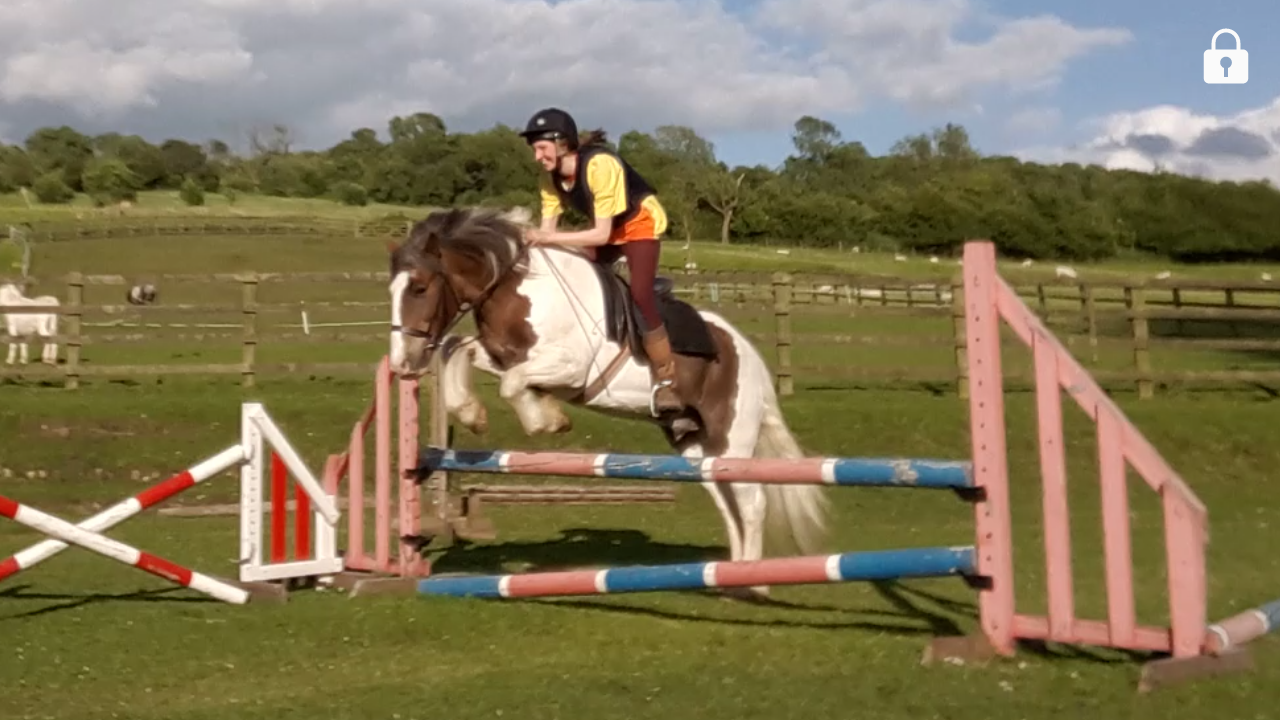
\includegraphics[width=\textwidth]{Figures/Harry}
\caption{Haribo}
\end{figure}

To begin validation and benchmarking of the nitrogen model, the pure nitrogen plasma will be used to take measurements of atomic nitrogen. 
The plasma parameters used experimentally can then be matched by the model and the experimental and simulated species densities can be compared.
For benchmarking, two-photon absorption laser induced fluorescence (TALIF) will be used, where a laser is used to excite nitrogen species so that fluorescence can be measured \todo{Check if TALIF will be used, timescale of laser etc}


\section{Planning of Experiments}
\subsection{Oxidative Stress Experiments}
method for looking at RNA expression

\future{Speak to Dmitris/read etc}

\subsection{COST jets}

COST jets are reference microplasma sources, designed to all be the same so that plasmas can be produced consistently by the different sources.
The four jets have all been investigated in terms of \todo{Find out what Fred has done}, and the aim is to carry out a simple bacterial killing assay, to determine the killing zone of each of the four jets so they can be compared. 

To do this, \textit{E. coli} MG1655 will be used. 
Bacteria will be grown, then plated onto agar plates, before being exposed to the plasma jet. 
The plates will then be incubated, and colonies counted and pictures taken, to determine the extent of the area of bacteria that has been killed by the plasma.

\subsubsection{Methods}
Blah blah blah.... This is how you grow bacteria.....

\section{Immediate Plans}
In the immediate future, an experiment for monitoring oxidative stress in skin cells needs to be developed. 
To do this, as well as the information from the literature review, I am also meeting with Dmitris Lagos, an RNA expert, to discuss the role of RNA in the stress response...


\section{Project Outlook}
















%\section{Oxidative Stress}
%Oxygen derived species - $\cdot$OH, O$_2^-\cdot$ and H$_2$O$_2$. However, O$_2^-\cdot$ and H$_2$O$_2$ have a low chemical reactivity, and do not readily react with biological molecules such as DNA, proteins and lipids. On the other hand, $\cdot$OH is very highly reactive, with reaction rates at or near diffusion-controlled rates for reactions with DNA \cite{Dizdaroglu2012oxidatively}.
%
%\subsection{DNA Damage}
%
%
%\section{Detecting Oxidative Stress - Bacteria}
%Different ways of detecting oxidative stress in bactera.
%In general, things to look for are cell death, membrane damage, DNA damage, lipid peroxidation and functional changes in proteins (e.g. enzyme deactivation).
%
%\subsection{Cell death}
%Measuring cell death can be done by measuring population level cell death, e.g through looking at zones of inhibition etc or at cellular level, e.g. using exclusion dyes.
%
%\subsection{Lipid Peroxidation}
%\begin{itemize}
%\item Lipid - large molecules made from smaller units of fatty acids and glycerol 
%\item Fatty acid - carboxylic acid consisting of a hydrocarbon chain and a terminal carboxyl group.
%\end{itemize}
%
%Radicals can attack polyunsaturated fatty acids and initiate lipid peroxidation in membranes.
%This can have significant effects on membrane fluidity and membrane-bound proteins.
%As a result of lipid peroxidation, aldehydes are often formed, which are long lived and able to function as "toxic second messenger" molecules, which can cause further damage to cells, in particular proteins \cite{Cabiscol2000oxidative}.
%These products include malonaldehyde (MDA) and 4-hydroxynonenal (HNE), which are particularly mutagenic and toxic, respectively \cite{Ayala2014lipid}.
%
%\subsection{DNA damage}
%
%\section{Methods}
%
%\begin{itemize}
%\item XTT assay. Metabolic activity
%
%Paper talking about oxidative stress in bacteria \cite{Cabiscol2000oxidative}. Talks about attack on lipids, proteins and DNA.
%
%\cite{Ezraty2017oxidative} is a paper with lots of biochemistry-y stuff in. Haven't read it - think it is a bit too in depth all about the mechanisms of protein damage, in particular sulphur containing side chains of proteins.
%
%\cite{Alkawareek2014potential} Paper looked at LTP interactions with bacteria, in particular bacterial killing/metabolism XTT assay (E. Coli, P. aeruginosa, B. cereus and MRSA), plasmid DNA damage (single and double strand breaks by looking whether the plasma was supercoiled (undamaged), open circular (single strand break) or linear (double strand break)), protein function (proteinase K's function was watched to see if the plasma was altering the structure in some way to prevent catalytic activity (it is pretty robust to changes in temp and pH therefore decrease in activity likely to be due to structural changes)), lipid peroxidation (MDA measurement in E. Coli) and membrane permeability (by measuring ATP leakage from E. Coli).
%\end{itemize}
%
%Assays:
%\begin{enumerate}
%\item \url{https://www.caymanchem.com/product/589320} - DNA/RNA Oxidative Damage ELISA Kit. Looks for 8-hydroxy-2'-deoxyguanosine from DNA, 8-hydroxyguanosine from RNA, and 8-hydroxyguanine from either DNA or RNA.
%\item
%\end{enumerate}
%%\section{}
%%\subsection{}
%
%\section{Detecting Oxidative Stress - Skin Cells}
%
%
%
%\section{Skin Models for Wound Healing Assays}
%Skin explants (people) can be cultured (as an organ culture) for up to 2 weeks at the air/liquid interface \cite{Gottrup2000models}.
%\subsection{Porcine Skin}
%
%\subsection{Hyaluronic Acid}
%
%\section{Cancer Things}
%\subsection{Radiotherapy}
%Radiation therapy can either be photon or particle, radiation.
%Photon radiation uses gamma ray or x ray beams focussed on the tumour, whereas particle radiation uses electrons, neutrons or protons for the same purpose - energy deposition into the tumour.
%By targeting the tumour with these beams, they deposit energy in the tumour cells, and cause ionisation of particles in the cells.
%This then leads to radical formation etc which causes damage to cancer cell DNA and prohibits their replication.
%Healthy cells are generally better at repairing DNA defects, meaning that if doses are delivered that cause sub-lethal levels of damage to healthy cells, then the healthy cells have time to repair before the next dose (as they divide much more slowly than cancer cells, so have longer to repair damage), whereas, cancer cells don't and therefore die.
%This gives specificity of a fashion.
%Damage to DNA occurs both directly (ie, the radiation directly damages the DNA), or indirectly, through formation of radical species which then attack the DNA. \cite{Baskar2012cancer}
%
%
%\subsection{Immunotherapy}
%\subsection{Photodynamic therapy}



\scriptsize
\bibliographystyle{ieeetr}
\bibliography{/Users/hld523/Bibliography/MyPapers}
\end{document}  